% !TEX root = main.tex

\begin{figure*}[t]
\centering
\begin{tabular}{@{}c@{}c@{}c@{}}

\includegraphics[width=0.25\textwidth]{speed-2p} & 

\includegraphics[width=0.25\textwidth]{speed-ip} & 

\includegraphics[width=0.25\textwidth]{speed-pni}
\end{tabular}
\vspace{-1mm}
\caption{Speed-up of our bidirectional sampler over a na\"ive sampler that performs KG traversal, on 2p, ip and pni query structures (\Figref{fig:query_tree}). Our bidirectional sampling is significantly more efficient than the baseline.
\label{fig:sampler_speed}}
\end{figure*}

\begin{table}[t]
\centering
\caption{Runtime performance on Freebase KG. *Results taken from ~\citet{mohoney2021marius} with the same GPUs. \label{tab:link_prediction}
}
\vspace{-3mm}
\resizebox{0.48\textwidth}{!}{%
    \begin{tabular}{c|c|ccc}
    \toprule
    \multirow{2}{*}{System} &  \multicolumn{4}{c}{Epoch Time (s)} \\
    & 1-GPU & 2-GPU & 4-GPU & 8-GPU  \\
    \hline
    Marius~\citep{mohoney2021marius}* & 727 &  - & - & - \\
    DGL-KE~\citep{zheng2020dgl}* & - & 1068 & 542 & 277 \\
    PBG~\citep{lerer2019pytorch}* & 3060 & 1400 & 515 & 419 \\
    \modelshort{} & 760 & 411 & 224 & 121 \\
    \bottomrule
    \end{tabular}
}
\end{table}

\begin{figure*}[t]
\centering
\begin{minipage}{0.615\textwidth}

\includegraphics[width=0.495\textwidth]{ogb-speedup}

\includegraphics[width=0.495\textwidth]{freebase-speedup}
\caption{\modelshort enjoys almost linear speed-up with respect to the number of GPUs, on both ogbl-wikikg2 and Freebase KGs, and across multiple embedding methods GQE, Q2B and BetaE. \label{fig:multigpu}}
\end{minipage}
\hfill
\begin{minipage}{0.38\textwidth}
\centering
\captionof{table}{Speed and GPU memory of \modelshort on the three large KGs with embedding dimension $=400$ and per device batch size $=512$. Our system design enables the (almost) graph-size agnostic speed and GPU memory usage.
\label{tab:largekgspeed} }
\vspace{-7mm}
\resizebox{0.98\textwidth}{!}{%
\begin{tabular}{c|c|c|cc|cc|cc}
\toprule 
Model & Dataset & Queries (x1K/Sec) & GPU Mem (MB) \\
\hline
\multirow{3}{*}{BetaE} &  FB400k & 123  & 1,872 \\
 & ogbl-wikikg2 & 121 & 1,860 \\
 & Freebase &  118 & 2,014 \\
\hline
\multirow{3}{*}{Q2B} &  FB400k & 135 & 1,796 \\
 & ogbl-wikikg2 & 130 & 1,776 \\
 & Freebase & 116 & 2,382 \\
 \hline
\multirow{3}{*}{GQE} &  FB400k & 189 & 1,726 \\
 & ogbl-wikikg2 & 195 & 1,750\\
 & Freebase & 188 & 2,056 \\
\bottomrule
\end{tabular}
}%
\end{minipage}
\end{figure*}


\section{Experimental results}\label{sec:exp}


Here we evaluate \modelshort on KG completion and multi-hop reasoning tasks on KG. The task is to answer multi-hop complex logical queries on KGs using various query embeddings. Besides the three small KGs used in prior works~\cite{ren2020query2box,ren2020beta}, we propose a novel set of multi-hop reasoning benchmarks on three extremely large KGs with more than 86 million nodes and 338 million edges. We first demonstrate the scalability of \modelshort on query sampling, multi-gpu speedup, GPU utilization over the three large KGs where all existing implementations fail. Additionally, we compare our single-hop KG completion runtime with state-of-the-art frameworks DGL-KE~\cite{zheng2020dgl}, Pytorch-Biggraph (PBG)~\cite{lerer2019pytorch} and Marius~\cite{mohoney2021marius}. Then we evaluate the end-to-end training performance of \modelshort on multi-hop reasoning over small as well as large KGs. This includes (1) calibration of the performance of three prior works GQE~\cite{hamilton2018embedding}, Q2B~\cite{ren2020query2box} and BetaE~\cite{ren2020beta} using \modelshort framework on the three small KGs; (2) a thorough evaluation of the query embedding models on the three large KGs where prior implementation~\cite{kgreasoning} is not applicable. 



\subsection{Experimental setup}

\textbf{Task setup.} Following the standard experimental setup~\citep{ren2020query2box}, given an incomplete KG, the goal is to train query embedding methods to discover missing answers of complex logical queries. The detailed task setup and training/validation/test split can be found in \appref{app:task-setup}.
Following the standard evaluation metrics, we adopt mean reciprocal rank (MRR) with the filtered setting as our metric. 
The detailed procedure of calculating the metrics can be found in~\appref{app:metrics}.


\textbf{Datasets.}
We used the three datasets FB15k, FB15k-237, NELL from \citet{ren2020beta}. These three KGs are small-scale with at most 60k entities.
To create a set of large-scale multi-hop KG reasoning benchmarks, we further sample queries on three large KGs: FB400k, ogbl-wikikg2 and Freebase. 
Ogbl-wikikg2 is a KG from the Open Graph Benchmark~\cite{hu2020open}. 
FB400k is a subset of Freebase~\cite{bollacker2008freebase} which is derived based on a knowledge graph question answering dataset ComplexWebQuestion (CWQ)~\cite{talmor2018web}. 
We further look at the complete Freebase KG used in DGL-KE. 
For FB15k, FB15k-237 and NELL, we directly take the validation and test queries from \citet{ren2020beta}.
For ogbl-wikikg2 and Freebase, we randomly sample validation and test queries using the official edge splits. We consider the same 14 query structures proposed in BetaE~\cite{ren2020beta}. For FB400k, we directly take the SPARQL annotations of the validation and test questions in the CWQ as our validation and test queries.
Statistics of all the datasets can be found in Table \ref{tab:meta_kg}. The KGs we use here are up to 1500$\times$ larger than those considered by prior work.

\textbf{Software and training details.}
We implement all models in Python 3.8 using Pytorch 1.9~\citep{paszke2019pytorch} with customized CUDA ops, and the samplers in C++ with multithreading. The machine has 8 NVIDIA V100 GPUs, 96x 2.00 GHz CPUs and 600GB RAM. All models have same embedding dimension for fair comparison.





\begin{figure}[t]
\centering
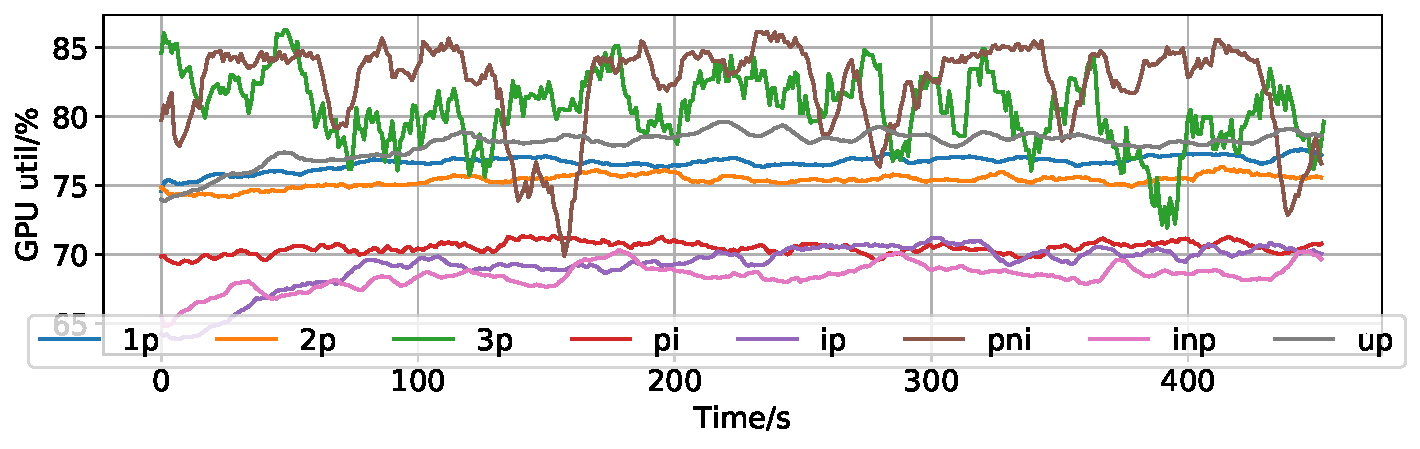
\includegraphics[width=0.48\textwidth]{figs/beta_gpu_util}
\vspace{-4mm}
\caption{GPU utilization with different query structures on Freebase with BetaE~\citep{ren2020beta}. \label{fig:gpu_util} }
\end{figure}

\begin{figure*}[h!]
\centering
\begin{minipage}{0.31\textwidth}
\centering
\captionof{table}{MRR results (\%) on large KGs with different methods all trained using \modelshort. 
Results for each query structure can be found in~\appref{app:detailedmrr}.
\label{tab:mergedmrr} 
}
\resizebox{1.0\textwidth}{!}{%
\begin{tabular}{c|ccc}
\toprule
{\small Dataset \textbackslash\: Model} & GQE & Q2B & BetaE\\
\hline
FB400k & 36.02 & {\bf 51.74} & 50.50 \\
ogbl-wikikg2 & 32.91 & 41.88 & \textbf{44.42} \\
Freebase & 80.71 & \textbf{85.67} & 84.33 \\
\bottomrule
\end{tabular}
}%
\end{minipage}
\hfill
\begin{minipage}{0.67\textwidth}
    \centering
    
\includegraphics[width=1.0\textwidth]{sampling.pdf}
    \vspace{-7mm}
    \caption{Accuracy (MRR) of different Q2B models trained using different samplers. We observe that our bidirectional sampler leads to more accurate models.
\label{fig:sampling_result} }
\end{minipage}
\end{figure*}

\subsection{Scalability}
\textbf{Speedup of bidirectional sampler.}
We verify the speed-up of the proposed bidirectional sampler over na\"ive exhaustive traversal one in \Figref{fig:sampler_speed} (more results on other query structures can be found in \appref{app:more_exp_results}). We test with different query structures where the bidirectional sampler is expected to achieve a square root reduction of the computation cost compared with traversal. We vary the constant $C$, \ie, the maximum expansion of each relation, and plot the time for sampling a minibatch of 1024 queries as the function of $C$ using the largest Freebase KG. We can see the exhaustive traversal approach runs out of the time limit quickly when $C$ grows, while our proposed sampler stays significantly more efficient across all query structures (\Figref{fig:query_tree}).


\textbf{GPU memory, utilization and end-to-end training speed.}
Here we show the scalability of \modelshort on all six KGs. We first compare \modelshort with prior implementation~\cite{kgreasoning} on the three small benchmark datasets created in \citet{ren2020beta}. As shown in the last two columns in Table~\ref{tab:calibrate}, \modelshort significantly improves the efficiency of end-to-end training of various query embeddings since \modelshort adopts a query sampling scheme that shares the negative samples for a sampled batch of queries. Specifically, \modelshort increases the speed by 119.4\% and reduces GPU memory usage by 30.6\% on average. Then we scale query embeddings up to the three large KGs. As shown in Table~\ref{tab:largekgspeed},  given the same embedding dimension and batch size, our system design allows for (almost) graph-size agnostic speed and GPU-memory usage across all methods.




In \Figref{fig:gpu_util} we further show the GPU utilization of BetaE model with different multi-hop query structures on Freebase. We plot the average utilization of 8 GPUs with smoothing of 10 seconds. More complex queries like \texttt{3p} and \texttt{pni} would have higher fluctuation due to the variance of sampling time. However as these queries also require more neural ops which in turn brings up the GPU utilization. Generally our system is able to keep a high GPU utilization for all these query structures.

\textbf{Multi-GPU speed up.}
We illustrate the speed-up of training on $\{$1, 2, 4, 8$\}$ GPUs with different methods on ogbl-wikikg2 and Freebase datasets in~\Figref{fig:multigpu}. Overall the speed grows almost linearly w.r.t. the number of GPUs, which shows the effectiveness of our asynchronous training and the communication overhead is negligible. Also the computationally heavier approaches like BetaE, which requires calculating KL-divergence between high-dimensional Beta distributions as well as its derivatives, benefit more from multi-GPU on \modelshort. 

\textbf{KG completion runtime.}
Here we compare the single-hop link prediction (KG completion) runtime performance with state-of-the-art large-scale KG frameworks including Marius, DGL-KE and PBG. We report the results for ComplEx model with 100 embedding dimension on Freebase. We use the same multi-GPU V100 configuration as in Marius, and the current official release versions are also the same. So for baseline results we reuse the table 7 from~\citet{mohoney2021marius}. As shown in Table~\ref{tab:link_prediction}, \modelshort achieves significantly faster runtime in 1-GPU setting than PBG, while being slightly slower than Marius. Also it scales better than the other systems, while Marius does not officially support multi-GPU parallel training functionality at the current stage. Given that \modelshort adopts the design choice of synchronized gradient update for dense parameters, and we do not partition the graph for the sake of multi-hop reasoning, it is nontrivial to be still comparable in the single-hop case.



\subsection{Predictive performance}
\textbf{Calibration on small KGs.}
We first calibrate our \modelshort system for GQE, Q2B, and BetaE on the three small benchmark datasets created in BetaE. As shown in Table~\ref{tab:calibrate}, \modelshort achieves overall comparable performance as the models trained on a fixed set of training queries using a single GPU. Specifically, \modelshort achieves comparable results for GQE and BetaE respectively but is able to further improve the performance of Q2B on FB15k with 3.54\% increase in MRR. 





\textbf{Query answering on large KGs.}
We also benchmark the embedding models on the three large KGs FB400k, ogbl-wikikg2 and Freebase. As shown in \tabref{tab:mergedmrr}, on ogbl-wikikg2, BetaE performs the best among all the other baselines. On both FB400k and Freebase, box embedding model Q2B achieves the best results. For all these methods, the baseline implementation~\cite{kgreasoning} cannot scale to such massive KGs due to the short of GPU memory and computationally expensive exhaustive query sampling. 
Our system \modelshort easily scales query embeddings to these large KGs using an asynchronous design with sparse embedding and optimizer. 
% 
The three KGs serve as an important benchmark for future multi-hop KG reasoning models.


\textbf{Performance with different samplers.}
We compare the performance of Q2B trained with different samplers, \ie, the na\"ive sampler (\texttt{exhaustive traversal}), bidirectional sampler (\texttt{bidirectional}) and randomly sampling KG entities as negative answers (\texttt{random}) on FB15k-237, FB400k and ogbl-wikikg2. As shown in \Figref{fig:sampling_result}, random sampling performs the worst since random negative sampling does not guarantee that the sampled entities are truly the negative (non-answer) entities. \texttt{bidirectional} performs comparable or even better than \texttt{exhaustive traversal}, as it can choose much larger $C$ during query sampling. Note that \texttt{exhaustive traversal} is very slow on large graphs, and it requires months for the baseline implementation with exhaustive traversal sampler to train a model with the same number of queries on ogbl-wikikg2.